% Figure: the bounded-degree gadget (Definition~\ref{def:bdeg}).
% Requires only tikz. Same colors as the gadget figure: rows vermillion, columns blue.
\begin{figure}[t]
\centering
\providecommand\Description[2][]{}%
\Description{Left: three tubes from three column surfaces meeting at a single orange row triangle. Right: the same row replaced by a horizontal pipe of four orange rings joined by annuli, each column surface tubed to its own ring, one surface sealed.}
\definecolor{bdRow}{HTML}{D55E00}%
\definecolor{bdCol}{HTML}{0072B2}%
\colorlet{bdLine}{bdCol!80!black}%
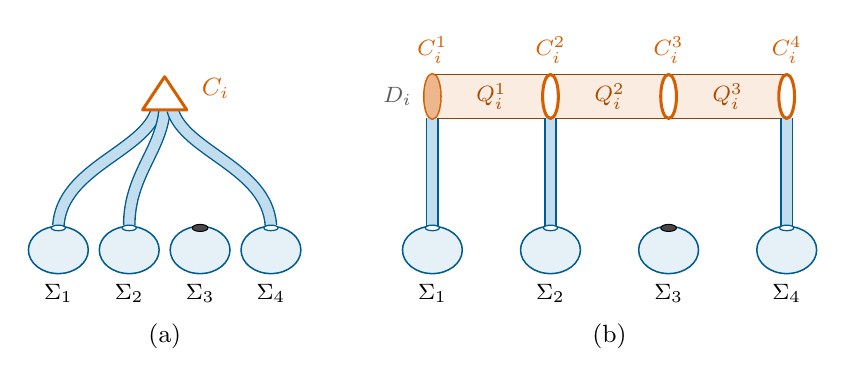
\begin{tikzpicture}[x=1cm,y=1cm,line join=round,
  surf/.style={fill=bdCol!10,draw=bdLine,line width=0.55pt},
  tube/.style={double=bdCol!24,double distance=3.6pt,line width=0.5pt,draw=bdLine},
  seal/.style={fill=black!72,draw=black,line width=0.35pt},
  hole/.style={fill=white,draw=bdLine,line width=0.45pt},
  rowcyc/.style={draw=bdRow,line width=1.1pt},
  lab/.style={font=\small},
  small/.style={font=\footnotesize}]
  % entries of row i: A_{i1}=1, A_{i2}=1, A_{i3}=0, A_{i4}=1
  %%% (a) the row cycle of Definition 4.2: all tubes of row i end on C_i
  \begin{scope}
    \draw[tube] (0.25,0.36) .. controls (0.3,1.1) and (1.35,1.3) .. (1.5,1.83);
    \draw[tube] (1.15,0.36) .. controls (1.15,1.0) and (1.55,1.3) .. (1.6,1.83);
    \draw[tube] (2.95,0.36) .. controls (2.9,1.1) and (1.85,1.3) .. (1.7,1.83);
    \foreach \x/\j in {0.25/1,1.15/2,2.05/3,2.95/4} {
      \draw[surf] (\x,0.05) ellipse (0.38 and 0.3);
      \node[small] at (\x,-0.5) {$\Sigma_{\j}$};
    }
    \foreach \x in {0.25,1.15,2.95} \draw[hole] (\x,0.33) ellipse (0.09 and 0.035);
    \draw[seal] (2.05,0.33) ellipse (0.1 and 0.045);
    \draw[rowcyc,fill=white] (1.32,1.83) -- (1.88,1.83) -- (1.6,2.25) -- cycle;
    \node[lab,text=bdRow,anchor=west] at (1.95,2.1) {$C_i$};
    \node[lab] at (1.6,-1.05) {(a)};
  \end{scope}
  %%% (b) the bounded-degree gadget: a chain of copies C_i^1,...,C_i^4 joined by annuli Q_i^j
  \begin{scope}[shift={(4.6,0)}]
    \def\cx{{0.4,1.9,3.4,4.9}}
    % the chain of annuli
    \fill[bdRow!12] (0.4,1.72) rectangle (4.9,2.28);
    \draw[bdRow!70!black,line width=0.5pt] (0.4,1.72) -- (4.9,1.72) (0.4,2.28) -- (4.9,2.28);
    \foreach \x/\j in {1.15/1,2.65/2,4.15/3} \node[small,text=bdRow!80!black] at (\x,2.0) {$Q_i^{\j}$};
    % tubes from the sockets of the 1-entries to their own copy
    \foreach \x in {0.4,1.9,4.9} \draw[tube] (\x,0.36) -- (\x,1.72);
    % copies: rings across the chain
    \foreach \x/\j in {0.4/1,1.9/2,3.4/3,4.9/4} {
      \draw[rowcyc,fill=white] (\x,2.0) ellipse (0.1 and 0.28);
      \node[small,text=bdRow,anchor=south] at (\x,2.3) {$C_i^{\j}$};
    }
    % the filling D_i of the first copy (row switch)
    \fill[bdRow!45] (0.4,2.0) ellipse (0.1 and 0.28);
    \node[small,text=black!65,anchor=east] at (0.26,2.0) {$D_i$};
    \foreach \x/\j in {0.4/1,1.9/2,3.4/3,4.9/4} {
      \draw[surf] (\x,0.05) ellipse (0.38 and 0.3);
      \node[small] at (\x,-0.5) {$\Sigma_{\j}$};
    }
    \foreach \x in {0.4,1.9,4.9} \draw[hole] (\x,0.33) ellipse (0.09 and 0.035);
    \draw[seal] (3.4,0.33) ellipse (0.1 and 0.045);
    \node[lab] at (2.65,-1.05) {(b)};
  \end{scope}
\end{tikzpicture}
\caption{Bounding the degree (Definition~\ref{def:bdeg}), shown for one row~$i$ with $A_{i1}=A_{i2}=A_{i4}=1$ and $A_{i3}=0$.
(a)~In the gadget of Definition~\ref{def:gadget}, all $\ell$ sockets of row~$i$ have a tube to the row cycle~$C_i$ in the universe (only the tubes of the $1$-entries are drawn), so every vertex of~$C_i$ lies in $\Theta(\ell)$ simplices.
(b)~In the bounded-degree gadget (here $\ell=4$), $C_i$ is replaced by a chain of copies $C_i^1,\dots,C_i^{\ell}$ joined by annuli~$Q_i^j$; the socket of position $(i,j)$ is tubed to its own copy~$C_i^j$, and the row switch $D_i$ fills the first copy.
Now every vertex of a copy lies in $O(1)$ simplices and every edge of a copy in at most three triangles, and the identity $\beta_2=|J|-\rk A[R,J]$ survives by telescoping along the chain (Lemma~\ref{lem:bdeg-crux}).}
\label{fig:bdeg}
\end{figure}
